%
% PKUMpLtX --- A LaTeX document class for 'Modern Physics Laboratory' in PKU based on `revtex4-2`
%
% Please read `README.md' and the template file before using
% 需要确保 font 选项指定的字体已安装! 具体参见 `README.md' 的说明.
\documentclass[font=default]{mpltx}

% 以下至 \begin{document} 都仅是本文件为了方便额外定义的命令, 写报告时不需要.
\hypersetup{colorlinks=true}% 超链接带颜色
\usepackage{xcolor}
\newcommand{\note}[1]{{\color{gray}#1}}
\NewDocumentCommand{\pkg}{s o m}{%
    \IfBooleanF{#1}{%
        \IfNoValueTF{#2}%
            {\href{https://www.ctan.org/pkg/#3}}%
            {\href{https://www.ctan.org/pkg/#2}}%
    }%
    {\textsf{#3}}%
}
\newcommand*\cs[1]{\texttt{\textbackslash #1}}
\newcommand*\env[1]{\textit{\texttt{#1}}}
\newcommand*\code[1]{\texttt{#1}}
\newcommand*\file[1]{\textbf{\texttt{#1}}}
\makeatletter
\newcommand\releasedate{%
    \href{https://github.com/CastleStar14654/PKUMpLtX/releases/tag/\mpltx@fileversion}%
        {\mpltx@filedate, \mpltx@fileversion}}
\makeatother
% 以上是本文件为了方便额外定义的命令, 写报告时不需要.

\begin{document}

\title{康普顿散射实验报告} % 切合报告内容, 简短明确, 可以不同于讲义
\author{李钰欣} % 这里 \emailphone 一定要紧跟在 \author 后方
\emailphone{2300011368@stu.pku.edu.cn}{(86)15816647600}
% 如果改用 \email 则仅需要邮箱参数
\affiliation{北京大学物理学院\quad 学号: 2300011368}
% % 可以使用 \zhdate 自动生成中文日期, 如
\date{\zhdate{2025/9/25}}
% % 也可使用 babel 的 \localedate, 如
% \date{\localedate{2020}{12}{1}}
% % 两者均会输出 `2020 年 12 月 1 日'
% 下面的 \date 的参数是为了自动输出正确版本号, 正式报告请替换为上面的两种 \date 之一
% \date{\releasedate}
\begin{abstract}
  本实验通过测量经过康普顿散射后不同角度下光子的光电峰峰位和光电峰面积,计算得到散射后光子的能量和微分散射截面。
  通过本实验验证了康普顿散射效应,即散射后光子的能量会随角度变化,散射后光子的微分截面会随角度变化。
\end{abstract}
\keywords{康普顿散射,NaI(Tl)探测器}

\maketitle

\section{引言}

康普顿散射指的是入射光子与物质原子中的核外电子产生非弹性碰撞而被散射的过程。
康普顿散射从实验上证实了光子是具有能量$E = \hbar \omega$和动量$p = \hbar k$的粒子,在微观的光子和电子的相互作用过程中,能量与动量守恒仍然成立。

 
\section{理论}\label{sec:theory}
1.康普顿散射

忽略电子的束缚能,视散射以前电子是静止的。由相对论的动量和能量守恒定律可以得到:
$hv' = \frac{hv}{1+ frac{hv}{m_0 c^2}(1-cos \theta)}$

2.康普顿散射的微分截面

微分截面定义:一个能量为h$v$的入射$\gamma$光子与原子中的一个核外电子作用后散射到$\theta$方向单位立体角里的概率,记作$\frac{d \sigma (\theta)}{d \Omega}$
本实验用NaIl(Tl)闪烁谱仪测量各散射角的散射$\gamma$光子能谱,由光电峰峰位及光电峰面积得出散射$\gamma$光子能量h$v'$,并计算出微分截面的相对值(相对$\theta = 20$°

\section{实验装置}
实验装置示意图 \autoref{fig:instrument2}

\begin{figure}
  \centering
  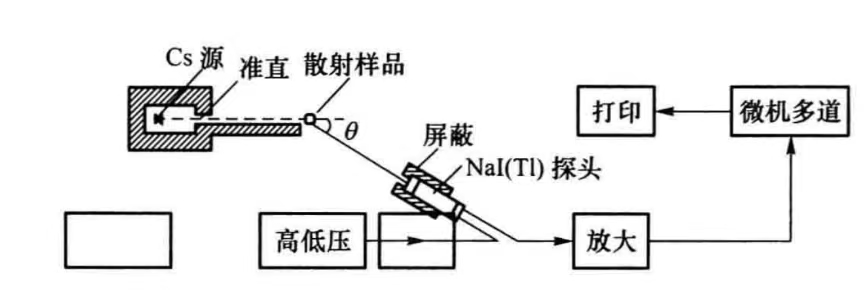
\includegraphics[width=0.85\linewidth]{fig/instrument2.jpg}
  \caption{康普顿散射实验装置示意图}
  \label{sec:instrument2}
\end{figure}

主要装置:康普顿散射实验台,铅棒($\phi = 20 mm$),
放射源($ ^{137}{Cs}$和$ ^{60}{Co}$),闪烁探测器,多道一体机,电脑

高压设置600V,放大倍数4.5。实验前需预热15min以上

\section{结果及讨论}
1.能量刻度

使用$ ^{137}{Cs}$测量0.662MeV光电峰位置及各参量,使用$ ^{60}{Co}$测量1.17MeV和1.33MeV光电峰位置及各参量,其中测量时间设为10min

测量结果:

\begin{table}[]
\begin{tabular}{llll}
能量(MeV)                & 道址                  \\
0.662                     & 459                    \\
1.17                      & 812                    \\
1.33                      & 916                     \\
\end{tabular}
\end{table}

数据处理: 

\begin{figure}
  \centering
  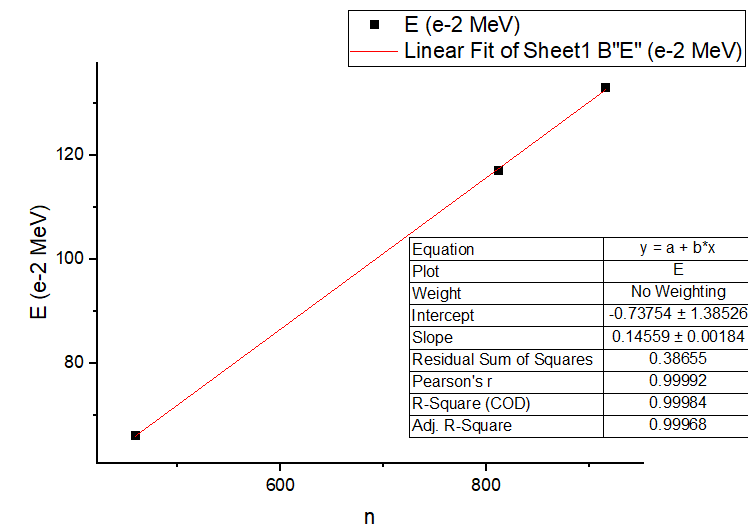
\includegraphics[width=0.85\linewidth]{fig/data2(1).png}
  \caption{能量刻度}
  \label{sec:data2(1)}
\end{figure}

即$E = {10}^{-3} \times (1.4559n - 7.3754)$,单位为MeV。

2.测量不同散射角时的散射光子能谱以及本底

插上散射铝棒,记录不同散射角时的道址,左右道位置和重点区面积。拔出散射铝棒,测量各角度对应相同道数区间的本底面积。

测量数据:
\begin{table}[]
\begin{tabular}{llll}
$\theta$(°)         & 道址                 &左道址            &右道址          &总面积    &本底面积    &净面积 \\
20                   & 421                  &389                &447            &14371    &846        &13525 \\
40                   & 346                   &320                &370           &9982     &417        &9565 \\
60                   & 266                   &245                &297           &8800     &421        &8379  \\
80                   & 219                  &191                  &239          &8169     &500        &7669  \\
100                  & 174                  &151                 &193           &8530     &615        &7915  \\
120                  &145                   &129                 &161           &9128     &709        &8419  \\
\end{tabular}
\end{table}

数据处理:

微分散射截面$\frac{d \sigma (\theta)}{d \Omega} = \frac{N_p(\theta)}{R(\theta)\eta(\theta)4 \pi N_0 N_e f}$,其中$N_p(\theta)$对应上表中净面积,
因此需求出$R(\theta)$和$\eta(\theta)$,之后才可求解相对散射截面。本实验设定$\theta_0$ = 20°。

根据课本数据,用最小二乘法得到:$R(\theta) =-0.71828 E(\theta) + 0.918046$,
$\eta(\theta) = 10^{-3} \times (-0.62907E(\theta) + 11.12064)$,其中E单位为MeV。

计算得各角度对应$R$,$\eta$,相对散射截面如下表:

\begin{table}[]
\begin{tabular}{llll}
$\theta$(°)         & 20                     &40                             &60                   &80                     &100                        &120 \\
E(keV)              & 605.559               &496.366                        &379.894                 &311.466              &245.951                 &203.730 \\
$R(\theta)$          & 0.4831                 &0.5615                           &0.6451              &0.6943                 &0.7413                    &0.7717 \\
$\eta(\theta)$     & $7.40 \times {10}^{-4}$  & $8.08 \times {10}^{-4}$  &$8.82 \times {10}^{-4}$ &$9.24 \times {10}^{-4}$  &$9.66 \times {10}^{-4}$     &$9.92 \times {10}^{-4}$    \\
相对微分截面          & 1                     &0.556729                         &0.389184               &0.315584            &0.292018                     &0.290421  \\
\end{tabular}
\end{table}

与课本数据对比:

\begin{figure}
  \centering
  \includegraphics[width=0.85\linewidth]{fig/figure_1.png}
  \caption{E- $\theta$}
  \label{sec:figure_1}
\end{figure}

\begin{figure}
  \centering
  \includegraphics[width=0.85\linewidth]{fig/figure_2.png}
  \caption{$\frac{d \sigma (\theta)}{d \Omega}$-$\theta$}
  \label{sec:figure_2}
\end{figure}

分析实验数据可以看到,实验所测能量略低于课本表格的能量,微分散射截面基本大于课本数据。

误差分析:

1.实验条件下,测量数据不对应某个准确的立体角,而对应该立体角附近一定展宽,因此微分散射截面偏大

2.在测量重点区面积时,由于仪器分辨率、测量时间等原因,在一定的道址范围内都能满足道计数为峰值约三分之一的标准,因此测量重点区面积会有误差,对微分散射截面测量带来误差。



\section{结论}
 本实验通过测量经过康普顿散射后光子的能量和相对微分散射截面,验证了康普顿散射效应,即散射后光子的能量会随角度变化,散射后光子的微分截面会随角度变化。
 通过本实验也对康普顿效应有了进一步的了解。


\end{document}





